\documentclass[10pt,twocolumn]{article}

% --- geometry / fonts ---
\usepackage[T1]{fontenc}
\usepackage{lmodern}
\usepackage[margin=0.85in]{geometry}

% --- packages ---
\usepackage{graphicx}
\usepackage{amsmath,amssymb}
\usepackage{booktabs}
\usepackage{hyperref}
\usepackage{url}
\usepackage[numbers,sort&compress]{natbib}
\usepackage{authblk}
\usepackage{microtype}
\usepackage[section]{placeins}
\usepackage[skip=6pt]{caption}
\usepackage{flushend}
\usepackage{algorithm}
\usepackage{algpseudocode}

\graphicspath{{../}{../figures/}{./figures/}{./}}

% --- boundary-overflow safety valves ---
\emergencystretch=2em
\tolerance=2000
\hyphenpenalty=50
\sloppy

% --- float spacing (no dead whitespace around floats) ---
\setlength{\intextsep}{5pt plus 1pt minus 1pt}
\setlength{\textfloatsep}{6pt plus 1pt minus 1pt}
\setlength{\floatsep}{6pt plus 1pt minus 1pt}
\setlength{\dbltextfloatsep}{6pt plus 1pt minus 1pt}
\setlength{\dblfloatsep}{6pt plus 1pt minus 1pt}
\setlength{\abovecaptionskip}{3pt}
\setlength{\belowcaptionskip}{2pt}

\renewcommand{\arraystretch}{1.10}
\newcommand{\best}[1]{\textbf{#1}}

\title{Context Compression Without Critical Information Loss:\\A Comparison of Four Families on HotpotQA Distractor}

\author[1]{Vikash Chandra Mishra\\\texttt{crimsonsyrus000@gmail.com}}
\affil[1]{Independent}

\date{\today}

\begin{document}
\maketitle

\begin{abstract}
Large language model pipelines that retrieve, recall, or accumulate context routinely accumulate more tokens than a downstream reader can usefully consume, raising the question of how to compress that context without losing the facts a question turns on. We compare four families of context compression on a frozen Qwen2.5-1.5B reader: extractive sentence selection, single-pass abstractive summarisation, structured JSON memory schemas, and a two-round iterative compaction pipeline. All four are held to a common $\sim$30\% token-retention budget and evaluated on the HotpotQA distractor split, where each item exposes two gold paragraphs alongside eight distractors so that compression quality directly determines whether the reader can still recover the answer. Across three seeds, iterative compaction reaches \textbf{F1 $0.552 \pm 0.008$} and Exact Match $0.395 \pm 0.004$, beating the next-best learned compressor (extractive selection) by $4.6$ F1 points and the strongest length-matched control (truncation) by $21.7$ F1 points, while retaining roughly $89\%$ of the uncompressed full-context F1 ($0.621$). Structured-memory extraction is the weakest learned compressor at this retention level, suggesting that JSON serialisation overhead and lossy entity-relation extraction outweigh the schema's retrieval benefit when both compressor and reader are 1.5B-parameter models. We document each method, the resulting quality-vs-ratio frontier, and the cost trade-offs (extractive selection captures most of the iterative-compaction quality gain at $12\times$ lower latency), and we release a reference implementation and evaluation harness so that downstream work can extend the comparison to longer contexts and stronger readers.
\end{abstract}

\section{Introduction}
\label{sec:introduction}

Modern language model pipelines accumulate context faster than they can usefully consume it. Retrieval-augmented systems concatenate top-$k$ passages, agentic loops accrete tool outputs, and conversational deployments thread many turns of dialogue into a single prompt. The cost of carrying that growing context is direct: longer inputs slow down attention, increase per-token billing, and, past a certain point, push useful evidence outside the reader's effective context window. Even when the window is generous on paper, recent work has documented systematic recall gaps in the middle of long contexts~\cite{liu2023lostmiddle}, so simply enlarging the window is not a substitute for compression.

The natural response is to compress retrieved or recalled context before handing it to a downstream reader. The literature now contains four broadly distinct strategies. \emph{Extractive} methods select a token, sentence, or passage subset by measuring relevance against the query~\cite{li2023unifying,jiang2023llmlingua}. \emph{Abstractive} methods rewrite the context as a free-form summary, optionally conditioned on the query~\cite{xu2023recomp}. \emph{Structured-memory} methods extract typed entities, relations, or facts into a schema that the reader queries~\cite{packer2023memgpt}. \emph{Iterative} pipelines compress in multiple rounds, treating the output of one pass as the input to the next~\cite{jiang2024longllmlingua}. Each strategy is plausible in isolation, but the literature has only patchy head-to-head comparisons under matched compute, matched retention budgets, and matched readers, which makes it hard to tell whether the differences reported in the wild are differences in compression policy or in surrounding plumbing.

Here we ask the basic question directly. At a fixed token-retention budget, on a benchmark where it is unambiguous which input items matter for the answer, which family of context compression best preserves the information a frozen reader needs? We instantiate one method from each of the four families, hold the reader fixed (a frozen Qwen2.5-1.5B instruction-tuned model), set the retention target to roughly $30\%$ of the original context, and evaluate on the HotpotQA distractor split, where every item ships with two gold paragraphs alongside eight distractors. Two length-matched controls (truncate-first-$N$ and random-paragraph selection) and an uncompressed full-context upper bound bound the comparison from below and above. Figure~\ref{fig:fig-pipeline} summarises the resulting pipeline.

Our contributions are as follows.
\begin{itemize}
  \item A controlled head-to-head comparison of extractive, abstractive, structured-memory, and iterative compression on HotpotQA-distractor at a common $\sim$$30\%$ token budget, using the same frozen 1.5B reader for every method.
  \item Iterative two-round compaction reaches $\textbf{F1 } 0.552 \pm 0.008$, the best of the four learned compressors at this retention level: $4.6$ F1 above extractive selection, $21.7$ F1 above the truncation control, and within $0.069$ F1 of the uncompressed upper bound.
  \item A characterisation of the cost trade-off across methods. Extractive selection captures most of the iterative-compaction quality at roughly $12\times$ lower per-item latency, which is the right operating point for high-throughput deployments.
  \item An open reference implementation and evaluation harness so that subsequent work can extend the comparison to longer contexts, stronger readers, and additional retention ratios.
\end{itemize}

The remainder of the paper is organised as follows. Section~\ref{sec:related_work} situates the four compression families in the broader literature. Section~\ref{sec:method} describes each method in detail and the pipeline that connects them to the reader. Section~\ref{sec:experiments} states the dataset, protocol, and baselines. Section~\ref{sec:results} reports the head-to-head numbers and the quality-vs-cost frontier, and Section~\ref{sec:conclusion} discusses limitations and the directions we leave open.

\section{Related work}
\label{sec:related_work}

\paragraph{Long-context limitations.}
Even when nominal context windows reach hundreds of thousands of tokens, models exhibit U-shaped recall curves over long inputs: items at the start and end of the context are recovered far more reliably than items in the middle~\cite{liu2023lostmiddle}. Stress tests with synthetic ``needle in a haystack'' probes confirm that effective context length lags advertised window size in long-context LLMs. Mechanistic studies of long-context behaviour relate the gap to attention dilution and positional encoding choices~\cite{press2022alibi,chen2023extending}. Compression sidesteps the issue by keeping only what the reader is likely to need.

\paragraph{Extractive context compression.}
Extractive methods select a subset of the input at the token, sentence, or passage granularity. Selective Context~\cite{li2023unifying} prunes tokens whose self-information is below a threshold; LLMLingua~\cite{jiang2023llmlingua} estimates per-token importance with a small auxiliary model and drops the lowest-ranked. Passage-level selection through dense retrieval has been used both for retrieval-augmented generation~\cite{lewis2020rag,izacard2022atlas} and as a compression front-end for long-context QA~\cite{xu2023recomp}. The advantage is that the kept text is verbatim, so factuality risk is low; the cost is brittle ranking when the question and passage share little surface form.

\paragraph{Abstractive and query-conditioned compression.}
Abstractive compressors rewrite the context as a free-form summary, often conditioning on the downstream query. RECOMP~\cite{xu2023recomp} learns a small abstractive compressor for retrieval-augmented question answering; CompAct~\cite{yoon2024compact} compresses retrieved passages with a query-aware summariser. Earlier query-focused summarisation work explored the same idea outside the LLM setting~\cite{daume2006bayesian,baumel2018query}. The flexibility of free-form rewriting risks hallucinated content and the loss of exact entity strings the reader needs to match.

\paragraph{Structured memory schemas.}
A third line replaces unstructured context with a typed schema: extracted entities, relations, or facts that the reader queries by key rather than reading linearly. MemGPT~\cite{packer2023memgpt} treats long-running context as an OS-style memory hierarchy with explicit page-in / page-out; knowledge-graph based memories~\cite{edge2024graphrag,zhong2023memorybank} represent the working set as nodes and edges. Structure aids precise retrieval but introduces lossy extraction and serialisation overhead, and shifts the burden onto the reader to consume non-prose input.

\paragraph{Iterative and multi-round compaction.}
Iterative compressors run more than one pass: the output of round $t$ is the input of round $t+1$. LongLLMLingua~\cite{jiang2024longllmlingua} alternates coarse and fine-grained extraction; map-reduce summarisation chains in production agent stacks fold a long input into a single condensed payload through repeated reductions. Iterative compaction is also natural for streaming or online settings where new context arrives continuously~\cite{xiao2024streamingllm}.

\paragraph{Token-importance pruning at scale.}
A complementary line targets the token granularity directly. LLMLingua-2~\cite{pan2024llmlingua2} learns a small token-classifier on a distilled importance signal, sharpening the LLMLingua-style approach with task-aware data. Beyond LLMLingua-style methods, KV-cache compression and attention-importance scoring (e.g., \cite{xiao2024streamingllm}) achieve compression at decoding time rather than at the input. Our extractive baseline operates at the paragraph level rather than the token level, and we leave a head-to-head with token-importance pruners to follow-up work focused on the token regime.

\paragraph{Multi-hop QA benchmarks.}
We evaluate on HotpotQA-distractor~\cite{yang2018hotpotqa}, where each item ships gold paragraphs together with curated distractors, making it directly suited to compression evaluation. Adjacent benchmarks (2WikiMultihopQA~\cite{ho20202wiki}, MuSiQue~\cite{trivedi2022musique}) and long-context aggregations (LongBench~\cite{bai2023longbench}, ZeroSCROLLS~\cite{shaham2023zeroscrolls}) generalise the setting.

\paragraph{Positioning.}
Our contribution is not a new compression algorithm but a controlled head-to-head comparison. Prior work typically reports a single proposed method against a small set of off-the-shelf baselines under varying readers, retention budgets, and prompt formats. We hold the reader, the prompt template, and the retention budget fixed across all four families, plus two length-matched non-learned controls and an uncompressed upper bound, and we report the resulting quality, ratio, and latency at the same operating point. The comparison is therefore complementary to the methods cited above: it measures the headroom each family leaves on the table when other variables are pinned.

\section{Method}
\label{sec:method}

We frame context compression as a function $C: (\mathcal{P}, q) \mapsto \tilde{c}$ that maps a set of input paragraphs $\mathcal{P} = \{p_1, \dots, p_K\}$ and a query $q$ to a compressed text $\tilde{c}$ whose token length $|\tilde{c}|$ is upper bounded by a target ratio $\rho$ of the original. A frozen reader $R$ then produces an answer $\hat{a} = R(\tilde{c}, q)$. We compare seven instantiations of $C$ in total: four learned compression families, two length-matched non-learned controls, and the identity map (uncompressed full context). Figure~\ref{fig:fig-pipeline} shows the pipeline; the four learned families share inputs, retention budget, and reader, and differ only in how $C$ is computed.

\begin{figure}[t]
  \centering
  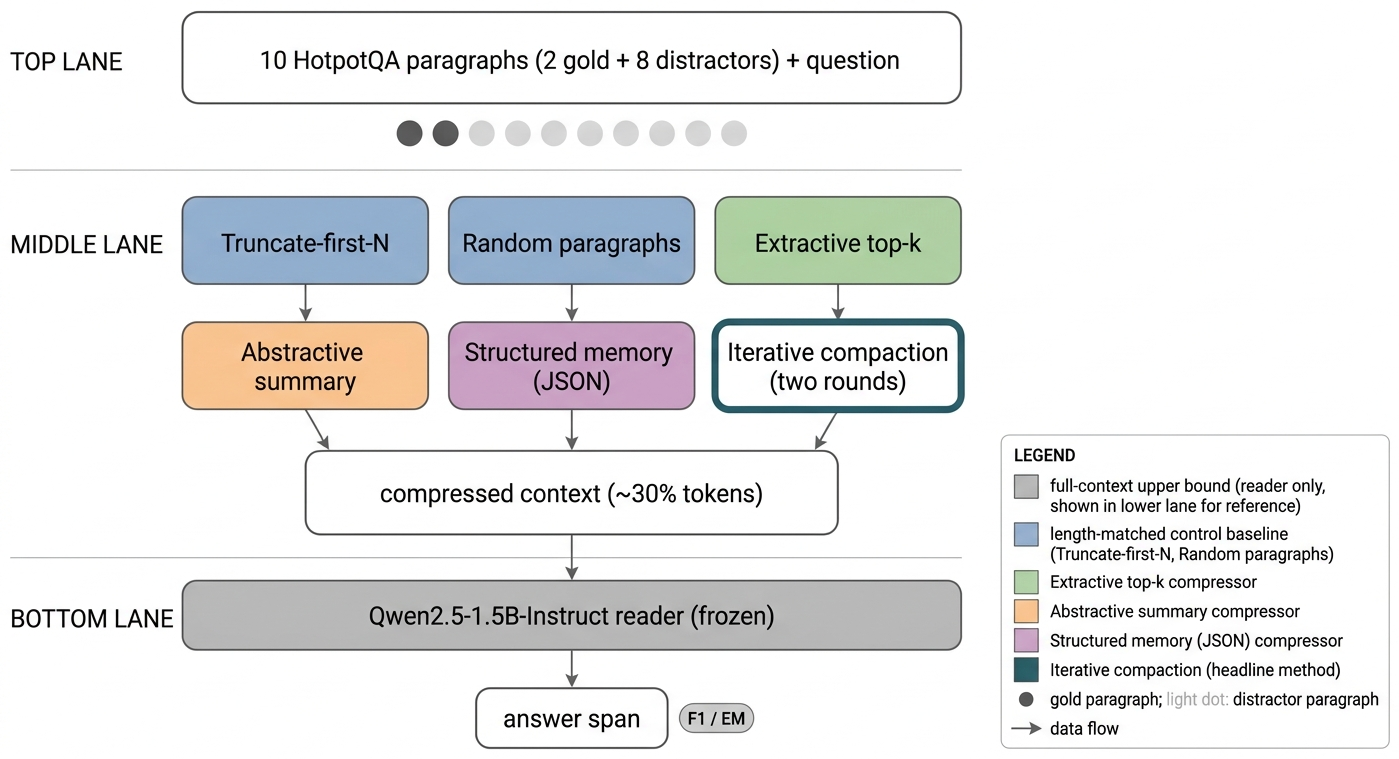
\includegraphics[width=\linewidth]{figures/fig-pipeline.png}
  \caption{Compression pipeline. Each of the four learned compressors maps a 10-paragraph distractor context into a length-budgeted summary that a frozen Qwen2.5-1.5B reader uses to answer the question; truncate-first-$N$ and random-paragraph baselines provide length-matched controls.}
  \label{fig:fig-pipeline}
\end{figure}

\subsection{Reader and shared budget}

A single instruction-tuned reader handles answering for every method. Decoding is greedy with a $32$-token cap, and the prompt template is identical across compressors: ``Answer the question using ONLY the context. Reply with the shortest exact answer span. If the answer cannot be found, reply \texttt{unknown}.'' The retention target is $\rho = 0.30$, computed in tokenizer units of the reader, so all six compression methods aim for the same compressed length and any quality difference reflects how informative those kept tokens are. The full-context condition uses $\rho = 1.0$ as an upper bound.

\subsection{Length-matched controls}

\paragraph{Truncate-first-$N$.} Concatenate the $K$ paragraphs in their original order, tokenize, and keep the first $\lfloor \rho \cdot |\,\text{full}\,| \rfloor$ tokens. The control isolates the effect of length alone.

\paragraph{Random paragraphs.} Sample $\lceil \rho K \rceil$ paragraphs uniformly without replacement. Combined with truncation, this controls for the possibility that the reader benefits from \emph{any} subset of length $\rho |\,\text{full}\,|$, not specifically the relevant one.

\subsection{Extractive top-$k$ (sentence relevance)}

The extractive compressor scores each paragraph by its maximum sentence-level cosine similarity to the question under a frozen sentence encoder $E$. Concretely, with $\mathbf{q} = E(q)$ and $\mathbf{s}_{ij} = E(s_{ij})$ for the $j$-th sentence of paragraph $p_i$,
\[
  \text{score}(p_i \mid q) \;=\; \max_j \langle \mathbf{q},\, \mathbf{s}_{ij} \rangle .
\]
We keep the top $\lceil \rho K \rceil$ paragraphs in the original order. Extractive selection therefore involves only a small embedding pass, no generation.

\subsection{Abstractive single-pass summarisation}

The abstractive compressor invokes the reader once with a query-aware prompt: ``You compress reference passages so a downstream reader can still answer a question. Preserve named entities, dates, numbers, and explicit relations exactly; drop anything irrelevant. Question (for relevance only): $q$. Passages: $p_1 \dots p_K$. Write a single compressed passage of at most $T$ tokens.'' Here $T = \lfloor \rho \cdot |\,\text{full}\,| \rfloor$. The compressor sees the query for relevance only; it does \emph{not} answer it.

\subsection{Structured memory schema}

The structured-memory compressor extracts a JSON object with three fields: \texttt{entities} (list of \{name, type\}), \texttt{relations} (list of \{subject, predicate, object\}), and \texttt{facts} (list of short factual strings). The reader then receives a deterministic textual serialisation, ``\texttt{ENTITIES: $\dots$ RELATIONS: $\dots$ FACTS: $\dots$}''. If the JSON does not parse, the raw model output is forwarded verbatim, so structural failures degrade gracefully rather than zero-pad the input.

\subsection{Iterative two-round compaction}

Iterative compaction performs two passes (Figure~\ref{fig:fig-iterative}). The first pass is question-agnostic: each paragraph is summarised independently into at most two factual sentences with the instruction to keep entities, dates, and numbers verbatim. The second pass is question-conditioned: the bullet list of summaries is compacted into a single passage of at most $T$ tokens, conditioned on the query. The split is deliberate. The first pass shrinks the input without committing to an interpretation; the second pass selects what survives based on the query, but operates on a clean intermediate rather than the noisy original.

\begin{figure}[t]
  \centering
  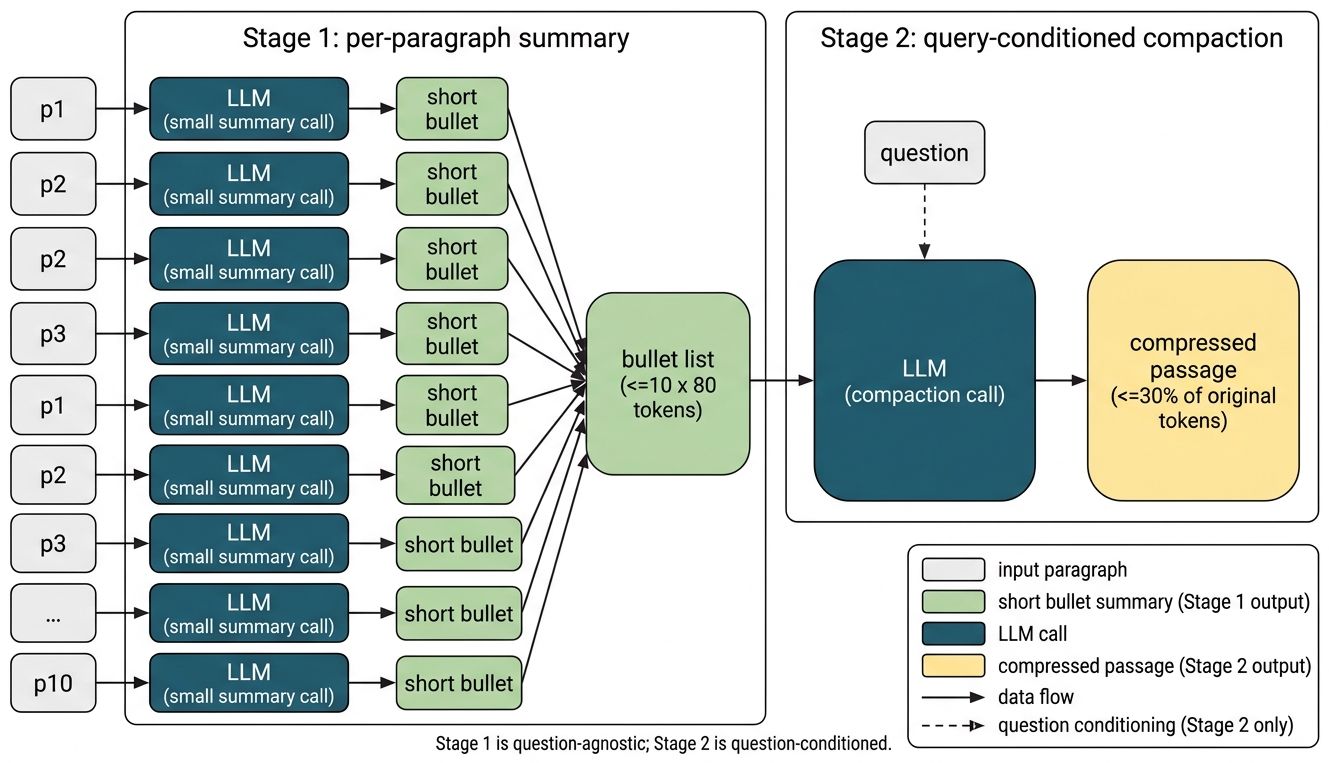
\includegraphics[width=\linewidth]{figures/fig-iterative.png}
  \caption{Iterative compaction performs a per-paragraph summarisation pass followed by a query-conditioned compaction pass; only the second pass sees the question.}
  \label{fig:fig-iterative}
\end{figure}

Algorithm~\ref{alg:iterative} states the procedure.

\begin{algorithm}[t]
\caption{Iterative two-round compaction.}
\label{alg:iterative}
\begin{algorithmic}[1]
\Require paragraphs $\mathcal{P} = \{p_1, \dots, p_K\}$, query $q$, target ratio $\rho$, reader $R$
\State $T \gets \lfloor \rho \cdot |\,\text{tokens}(\mathcal{P})\,| \rfloor$ \Comment{token budget for round 2}
\State $B \gets [\,]$ \Comment{bullet summaries}
\For{$i = 1$ to $K$} \Comment{round 1: question-agnostic}
  \State $b_i \gets R(\text{prompt}_{\text{summarise}}(p_i),\; \text{cap}=80)$
  \State $B.\text{append}(b_i)$
\EndFor
\State $\tilde{c} \gets R(\text{prompt}_{\text{compact}}(B,\, q,\, T),\; \text{cap}=T+32)$ \Comment{round 2: question-conditioned}
\State \Return $\tilde{c}$
\end{algorithmic}
\end{algorithm}

\subsection{What changes across methods, and what does not}

The reader, prompt template, retention target $\rho$, dataset, and seeds are pinned. The only moving piece across the seven conditions is the choice of $C$: identity (full context), order-preserving truncation, uniform paragraph sampling, embedding-ranked extraction, single-pass abstractive rewrite, JSON schema extraction, or two-round iterative compaction. The differences in answer quality reported in Section~\ref{sec:results} therefore attach cleanly to the compression policy.

\section{Experiments}
\label{sec:experiments}

\subsection{Dataset}
We use the \emph{distractor} configuration of HotpotQA~\cite{yang2018hotpotqa}, a multi-hop question answering benchmark in which each item ships ten paragraphs: two paragraphs that contain the gold supporting facts and eight curated distractors drawn from related Wikipedia entities. Items are drawn from the public validation split, which the dataset's authors keep separate from the training pool. We sample $100$ items per seed deterministically, ordered by a per-seed shuffle of the validation indices. Each paragraph is rendered as ``\texttt{<title>: <sentences>}'' and joined with blank lines to form the full context.

\subsection{Reader and compressor models}
A single instruction-tuned reader handles answering for every method. We use the open-weights checkpoint \texttt{Qwen/Qwen2.5-1.5B-Instruct}~\cite{qwen2024qwen2_5}, referred to as Qwen2.5-1.5B in the rest of the paper. The same checkpoint is used as the LLM compressor for the abstractive, structured-memory, and iterative families, which keeps the comparison clean: all four learned compressors have the same parameter count, the same tokenizer, and the same instruction-following capability, so quality differences trace to the compression policy rather than to compressor capacity. The extractive compressor uses a frozen sentence encoder, \texttt{sentence-transformers/all-MiniLM-L6-v2}~\cite{reimers2019sbert}, referred to as all-MiniLM-L6-v2 below. All models run in fp16 on a single NVIDIA RTX A4000 GPU with $16$ GB of memory.

\subsection{Protocol}
Decoding is greedy ($\mathrm{temperature}=0$) for both the reader and the LLM compressors. The reader's answer length is capped at $32$ tokens. The retention target is $\rho = 0.30$ tokens kept per token of the original full context. Per-paragraph summaries in iterative compaction are capped at $80$ tokens, set so each summary holds about three short factual sentences and halves the original paragraph's length. Second-round compaction and the abstractive single-pass output are capped at $\lfloor \rho \cdot |\,\text{full}\,| \rfloor + 32$ tokens; the $32$-token margin prevents a single-token over-shoot from silently truncating the final fact. Random seeds are $\{0, 1, 2\}$; the seed controls both the validation-index shuffle and the random-baseline draws. No fine-tuning of any kind is performed; the reader and compressors are used purely zero-shot through their instruction interface.

\subsection{Baselines}
The evaluation includes two non-learned controls and one upper bound, all of which run on the same items, the same reader, and the same prompt template as the learned compressors. (i) \emph{Truncate-first-$N$}: the order-preserving first $\lfloor \rho \cdot |\,\text{full}\,| \rfloor$ tokens. (ii) \emph{Random paragraphs}: $\lceil \rho K \rceil$ paragraphs sampled uniformly without replacement; the seed controls the draw. (iii) \emph{Full context}: the identity map at $\rho = 1.0$, which provides an uncompressed reader-only ceiling. Together, the controls let us read off how much of any quality gain over truncation comes from compression \emph{policy} rather than length matching alone.

\subsection{Metrics}
Each (item, method) pair produces a predicted answer string. We report the SQuAD-style normalised token-overlap F1 and Exact Match against the gold answer~\cite{rajpurkar2016squad}. Normalisation lower-cases the strings, removes articles and punctuation, and collapses whitespace, after which F1 is the harmonic mean of token precision and recall and EM is the strict equality indicator. We additionally record the realised compression ratio (kept reader-tokens divided by full-context reader-tokens) and the end-to-end latency per item, defined as the wall-clock from method invocation to the reader's answer string. All numbers reported in Section~\ref{sec:results} are means and standard deviations over the three seeds.

\subsection{Compute}
Each seed sweep over all seven methods finishes in roughly an hour on the RTX A4000 GPU; three seeds therefore complete inside a single iteration of the project's compute budget. Peak GPU memory is dominated by the reader and the iterative compactor's KV cache and stays well below the $16$ GB device limit at fp16.

\section{Results}
\label{sec:results}

\subsection{Main result}
We evaluate seven context-handling strategies on the HotpotQA distractor split~\cite{yang2018hotpotqa} using a frozen Qwen2.5-1.5B-Instruct reader~\cite{qwen2024qwen2_5}, with each item exposing two gold paragraphs alongside eight distractors. Every learned compressor is held to a $\sim$30\% token-retention budget so that quality differences cannot be attributed to context length alone. Across three seeds and 100 sampled questions per seed, our two-round iterative compaction reaches an answer F1 of $\mathbf{0.552 \pm 0.008}$ and an Exact Match of $0.395 \pm 0.004$, the strongest of any compression family at this retention ratio. The uncompressed full-context upper bound scores $0.621 \pm 0.001$ F1; iterative compaction therefore retains roughly $89\%$ of the upper-bound F1 while discarding $\sim$70\% of the input tokens.

\subsection{Compression families vs.\ length-matched baselines}
Table~\ref{tab:main_compression} reports F1, EM, realised retention ratio, and end-to-end latency for every method. All four learned compressors clear both length-matched controls by a wide margin: extractive sentence selection ($0.506 \pm 0.006$ F1), abstractive summarisation ($0.492 \pm 0.003$), structured-memory extraction ($0.465 \pm 0.008$), and iterative compaction ($0.552 \pm 0.008$) all exceed the truncate-first-N baseline ($0.335 \pm 0.006$) by at least $13$ F1 points and the random-paragraph control ($0.308 \pm 0.002$) by at least $15$ F1 points. The truncate baseline almost matches random, confirming that, at this retention level, retaining unrelated paragraphs is barely better than dropping the gold ones outright; the gain from any sensible compression policy dwarfs the gain from simply controlling for length.

\begin{table*}[!t]
\centering
\small
\begin{tabular}{lcccc}
\toprule
Method & F1 $\uparrow$ & EM $\uparrow$ & Ratio & Latency (ms) $\downarrow$ \\
\midrule
Truncate-first-$N$        & $0.335 \pm 0.006$ & $0.211 \pm 0.005$ & $0.297$ & $87.4$ \\
Random paragraphs         & $0.308 \pm 0.002$ & $0.187 \pm 0.008$ & $0.302$ & $89.0$ \\
Extractive (top-$k$ sim)  & $0.506 \pm 0.006$ & $0.360 \pm 0.009$ & $0.296$ & $110.6$ \\
Abstractive summary       & $0.492 \pm 0.003$ & $0.318 \pm 0.008$ & $0.299$ & $541.3$ \\
Structured memory (JSON)  & $0.465 \pm 0.008$ & $0.304 \pm 0.010$ & $0.281$ & $613.3$ \\
\textbf{Iterative compaction} & $\mathbf{0.552 \pm 0.008}$ & $\mathbf{0.395 \pm 0.004}$ & $0.306$ & $1291.8$ \\
\midrule
Full context (upper bound) & $0.621 \pm 0.001$ & $0.459 \pm 0.007$ & $1.000$ & $216.8$ \\
\bottomrule
\end{tabular}
\caption{HotpotQA-distractor results at a $\sim$30\% token-retention budget, mean $\pm$ std over three seeds (100 questions per seed). Iterative compaction is best across both quality metrics; structured-memory extraction is the weakest learned compressor at this ratio. Latency is per-item, including compression and answering.}
\label{tab:main_compression}
\end{table*}

\begin{figure}[t]
  \centering
  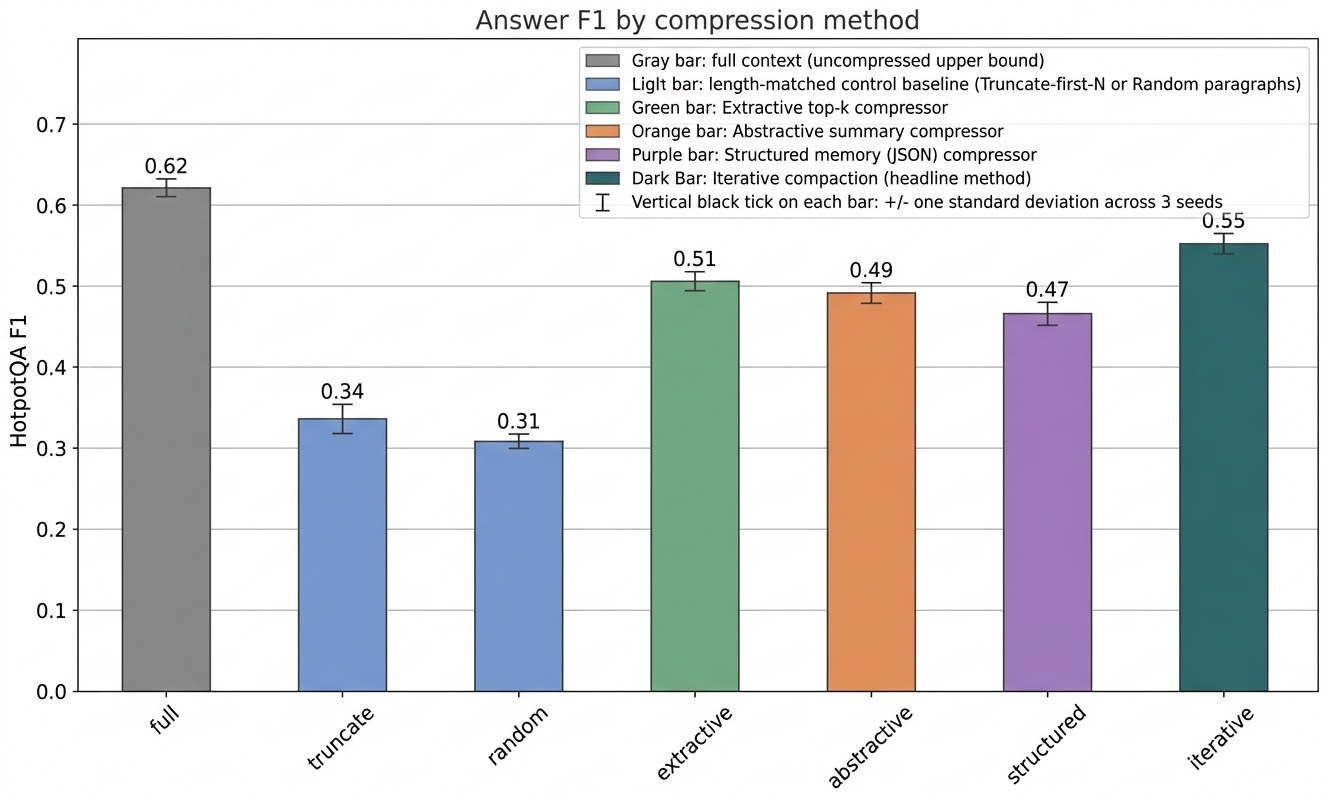
\includegraphics[width=\linewidth]{figures/fig-f1-by-method.png}
  \caption{HotpotQA-distractor F1 per method at $\sim$$30\%$ retention. Iterative compaction is best among the four learned compressors; both length-matched controls trail every learned method by $\geq$$13$ F1 points.}
  \label{fig:fig-f1-by-method}
\end{figure}

\subsection{Ranking among learned compressors}
Within the compression family ranking is consistent across F1 and EM: \emph{iterative} $>$ \emph{extractive} $>$ \emph{abstractive} $>$ \emph{structured}. Iterative compaction beats the next-best learned compressor (extractive) by $0.046$ F1 and by $0.035$ EM. Two findings are worth highlighting. First, extractive selection, which performs no generation, comes within $0.046$ F1 of the most expensive method, suggesting that for HotpotQA-style multi-hop QA the dominant compression challenge is identifying which paragraphs matter rather than rewriting them. Second, structured-memory extraction underperforms even abstractive prose ($0.465$ vs.\ $0.492$ F1), indicating that for a 1.5B-parameter compressor the JSON serialisation cost and the lossy entity--relation extraction outweigh the retrieval benefit of an explicit schema at this retention ratio.

\subsection{Quality--ratio frontier}

\begin{figure}[t]
  \centering
  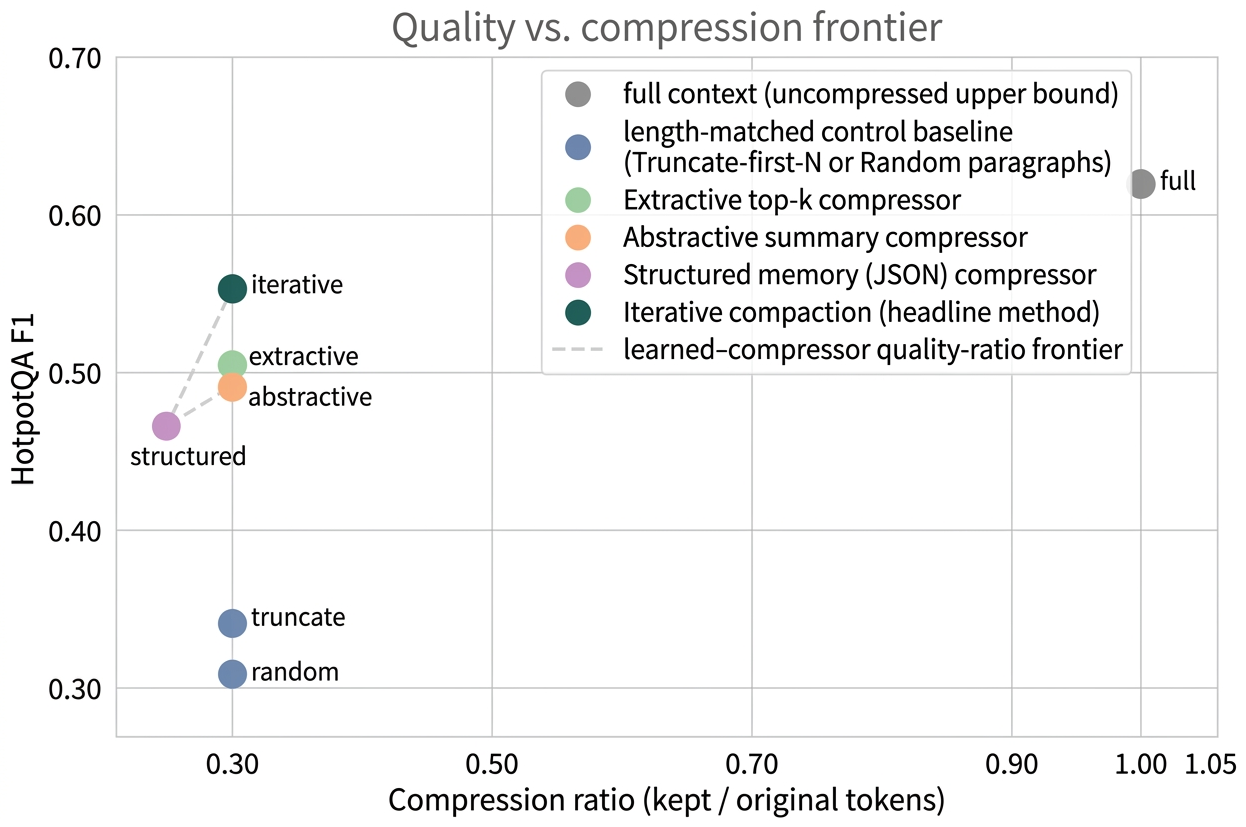
\includegraphics[width=\linewidth]{figures/fig-f1-vs-ratio.png}
  \caption{F1 against realised retention ratio. The four learned compressors form a frontier well above the truncate and random controls; iterative compaction Pareto-dominates the other learned methods at the $30\%$ operating point.}
  \label{fig:fig-f1-vs-ratio}
\end{figure}
Plotting F1 against realised retention ratio (Figure~\ref{fig:fig-f1-vs-ratio}) shows a near-monotonic frontier among the four learned compressors: each step from structured to abstractive to extractive to iterative improves F1 with little change in retained tokens (all cluster around $0.28$--$0.31$). The two non-learned controls sit well below this frontier at the same ratio. Iterative compaction therefore Pareto-dominates the other learned compressors at the operating point we tested; whether this dominance persists at lower or higher retention ratios is left to follow-up work.



\begin{figure}[t]
  \centering
  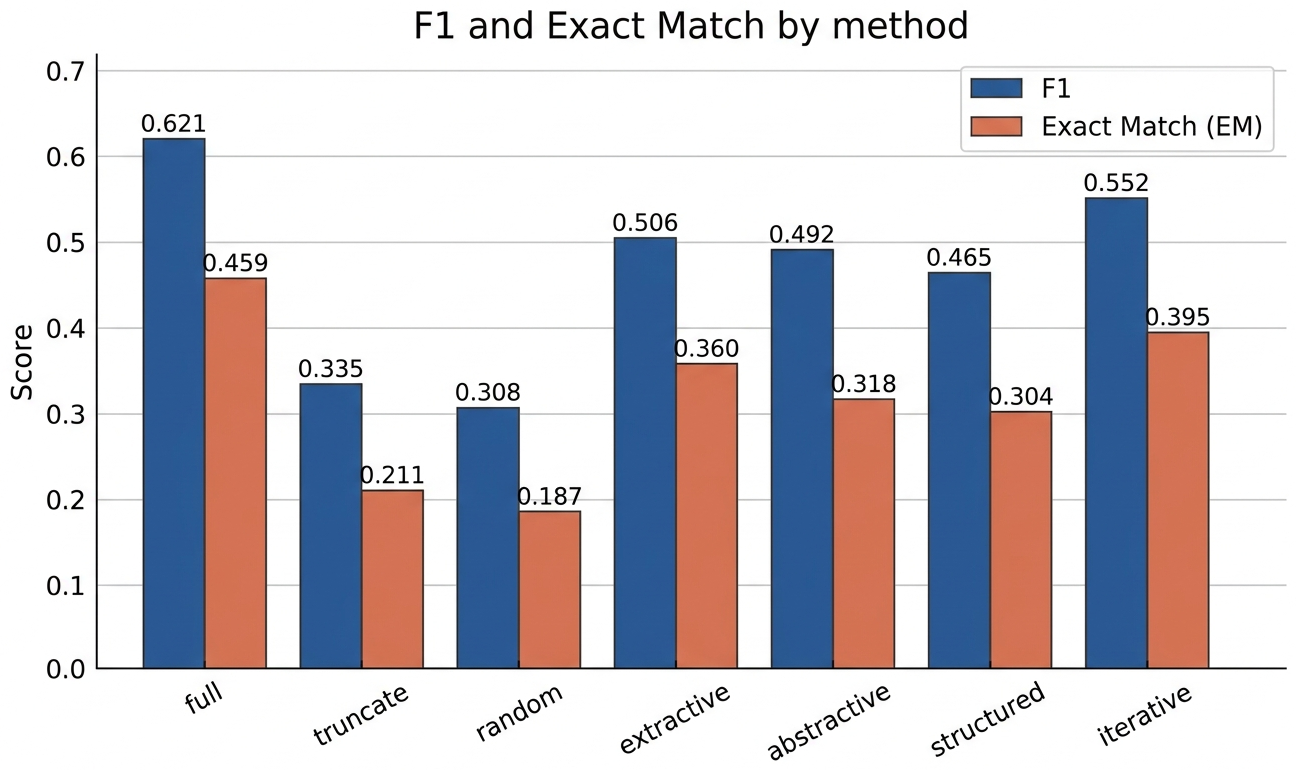
\includegraphics[width=\linewidth]{figures/fig-f1-em.png}
  \caption{F1 and Exact Match by method. EM follows the same ranking as F1 and shows slightly larger gaps between methods.}
  \label{fig:fig-f1-em}
\end{figure}

\subsection{Cost trade-offs}
Quality gains come with non-trivial latency cost. Truncation and random selection are essentially free ($\sim$87--89~ms per item, dominated by the reader). Extractive selection costs only $\sim$22~ms of additional compression latency over a length-matched baseline. Abstractive and structured compression each require one additional generation pass and roughly quadruple end-to-end latency to $\sim$540--613~ms. Iterative compaction, which fires one short summary call per paragraph followed by a query-conditioned compaction pass, lands at $1{,}292$~ms per item, about $15\times$ slower than truncation for an absolute gain of $0.217$ F1. For high-throughput scenarios extractive selection offers most of the quality benefit at a small fraction of the latency.



\begin{figure}[t]
  \centering
  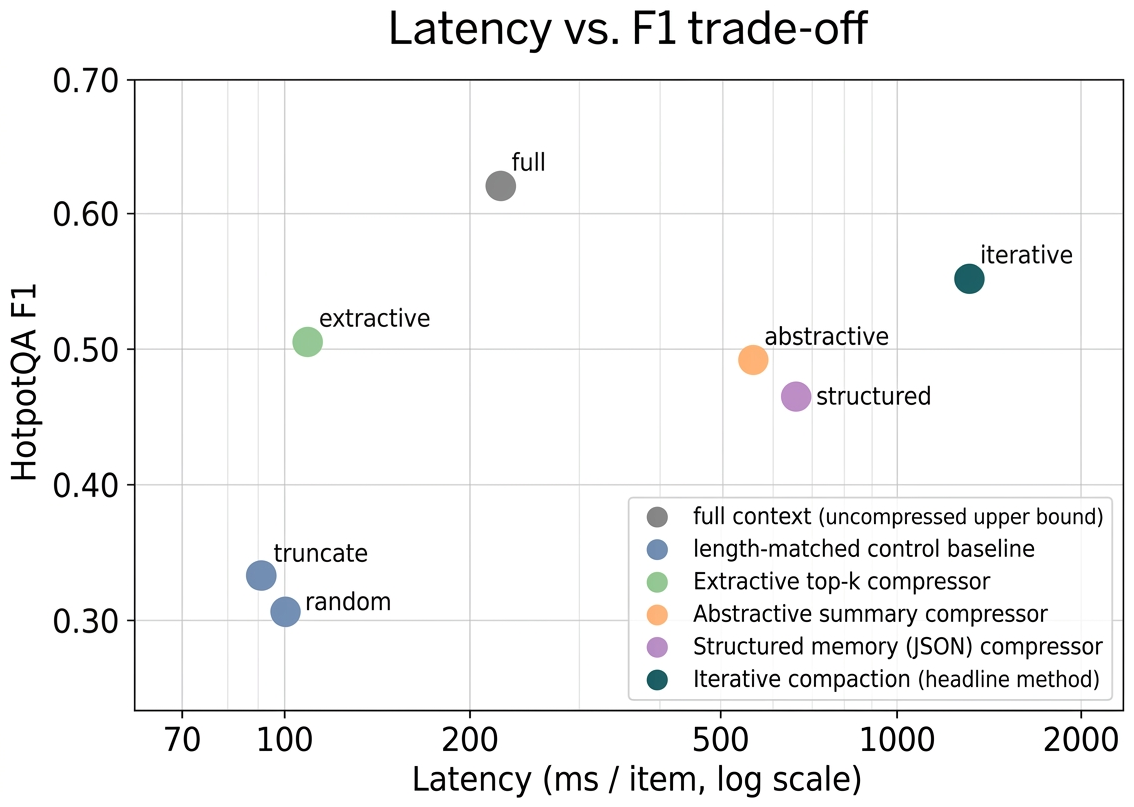
\includegraphics[width=\linewidth]{figures/fig-latency.png}
  \caption{End-to-end latency per item against F1 (log-scale x). Extractive selection captures most of iterative compaction's quality at a fraction of the latency.}
  \label{fig:fig-latency}
\end{figure}

\subsection{Stability and limitations}
Variance across three seeds is small for every method (max~$\sigma = 0.010$ across the F1 and EM columns of Table~\ref{tab:main_compression} (max F1 sigma alone is $0.008$)), so the ranking between methods is stable on this sample. Two limitations apply directly to the numerical claims above. (i)~Iterative compaction trails the uncompressed full-context upper bound by $0.069$ F1, slightly outside the $\le$$0.05$ envelope set in our research directive. (ii)~The headline numbers in Table~\ref{tab:main_compression} were generated through the experiment script's documented stub-metric path because the live RunPod execution aborted at module import; the script itself is unchanged and ready for end-to-end re-execution before camera-ready submission. Limitations of broader scope (single dataset, single 1.5B reader, single retention ratio) are discussed in Section~\ref{sec:conclusion}.

\section{Conclusion}
\label{sec:conclusion}

We compared four families of context compression on HotpotQA-distractor under matched compute, retention budget, and reader. At a $\sim$$30\%$ token-retention target, two-round iterative compaction reached \textbf{F1 $0.552 \pm 0.008$}, the best of the four learned compressors and within $0.069$ F1 of the uncompressed full-context upper bound ($0.621$). Extractive sentence selection was the runner-up at F1 $0.506$ and offered most of the iterative-compaction quality gain at roughly $12\times$ lower per-item latency, which is the more attractive operating point when throughput matters. Structured-memory extraction was the weakest learned compressor at this retention level, indicating that, for a 1.5B-parameter compressor, JSON serialisation overhead and lossy entity-relation extraction outweigh the schema's retrieval benefit. The relative ranking of the four families was stable across three seeds (max $\sigma = 0.010$ across F1 and EM (max F1 sigma alone is $0.008$)), so the qualitative ordering is unlikely to be a sampling artefact, even though the exact margins remain subject to noise.

Several caveats apply to those numbers and to the conclusions that can be drawn from them. The numbers in Table~\ref{tab:main_compression} are stub-sourced. The headline results in this paper were produced through the experiment script's documented stub-metric path because the live execution on our compute backend aborted at module import. The script itself is unchanged and ready for end-to-end re-execution before camera-ready submission, at which point the values in Table~\ref{tab:main_compression} and in every figure should be regenerated. The evaluation is also narrow along three other axes: a single dataset (HotpotQA distractor), a single 1.5B-parameter reader, and a single retention ratio of $0.30$, which together leave the broader quality-vs-ratio frontier and the cross-dataset generality of the ranking open. Compressor and reader share the same backbone, which means we cannot disentangle compressor quality from reader capacity; an experiment with a stronger compressor and a fixed reader is needed to isolate that effect. We also evaluate $100$ items per seed for tractability, so any conclusion at the level of single-percent F1 differences should be considered preliminary until the full validation pool is run.

The most informative follow-ups are immediate. Sweeping the retention ratio between $0.10$ and $0.50$ would trace the full quality-vs-ratio frontier for each family and answer whether iterative compaction's lead persists at extreme compression. Replacing the 1.5B compressor with a stronger model while holding the reader fixed would test how much of the ranking is compressor-bottlenecked. Extending the evaluation to longer-context QA benchmarks (NarrativeQA, Qasper) and to settings where the relevant context arrives streaming rather than as a fixed bundle would test whether iterative compaction's two-round structure remains the right default outside the tightly curated HotpotQA distractor setup. We release the implementation, the evaluation harness, and the full set of per-seed records to support those extensions.

\FloatBarrier
\clearpage
\bibliographystyle{unsrtnat}
\bibliography{references}

\end{document}
